% Compilar desde esta carpeta: pdflatex -interaction=nonstopmode -halt-on-error clase12_perceptron_lineal.tex
% Repetir la compilación para actualizar referencias y numeración.
% Estilo adaptado de DL_MRI_class/DL_MRI_presentation.tex (Evelyn Cueva).
\documentclass[10pt,aspectratio=169,xcolor={dvipsnames}]{beamer}
\usepackage[utf8]{inputenc}
\usepackage[T1]{fontenc}
\usepackage{lmodern}
\usepackage[spanish,es-nodecimaldot]{babel}
\usepackage{amsmath,amssymb,bm}
\usepackage{graphicx,booktabs,tikz,listings}
\usetikzlibrary{arrows.meta,positioning,calc}
\graphicspath{{figuras/}}

% Paleta, títulos y recuadros del material DL_MRI_class.
\definecolor{fondo}{RGB}{18,49,90}
\definecolor{verde}{HTML}{087F6B}
\definecolor{naranja}{HTML}{D65324}
\setbeamercolor{normal text}{fg=fondo,bg=white}
\setbeamercolor{math text}{fg=black!75}
\setbeamercolor{structure}{fg=fondo}
\setbeamercolor{frametitle}{fg=fondo,bg=white}
\setbeamercolor{bottombox}{fg=fondo,bg=white}
\setbeamercolor{lgraybox}{fg=fondo,bg=gray!10}
\setbeamercolor{yellowbox}{fg=fondo,bg=yellow!17}
\setbeamercolor{greenbox}{fg=fondo,bg=verde!10}
\setbeamercolor{orangebox}{fg=fondo,bg=naranja!10}
\setbeamercolor{section title}{fg=fondo,bg=white}
\setbeamercolor{itemize item}{fg=fondo}
\setbeamertemplate{itemize items}[circle]
\setbeamertemplate{navigation symbols}{}
\setbeamersize{text margin left=8mm,text margin right=8mm}
\setbeamertemplate{frametitle}{\vspace{2mm}\color{fondo}\bfseries\insertframetitle\par\vspace{-2mm}\rule{\textwidth}{0.4pt}}
\setbeamertemplate{footline}{%
    \leavevmode\hbox{%
    \begin{beamercolorbox}[wd=.23\paperwidth,ht=2.5ex,dp=1ex,center]{bottombox}
        \insertshortauthor
    \end{beamercolorbox}%
    \begin{beamercolorbox}[wd=.46\paperwidth,ht=2.5ex,dp=1ex,center]{bottombox}
        \insertshorttitle
    \end{beamercolorbox}%
    \begin{beamercolorbox}[wd=.31\paperwidth,ht=2.5ex,dp=1ex,right]{bottombox}
        \insertshortdate\hspace{1.5em}\insertframenumber/\inserttotalframenumber\hspace{2ex}
    \end{beamercolorbox}}\vskip2pt}
\newcommand{\tcg}[1]{\textcolor{verde}{#1}}
\newcommand{\tcr}[1]{\textcolor{naranja}{#1}}
\newenvironment{caja}[1][lgraybox]{\begin{beamercolorbox}[sep=0.7em,wd=\linewidth]{#1}}{\end{beamercolorbox}}
\newcommand{\actividad}[2]{\begin{caja}[yellowbox]\textbf{#1}\par\smallskip #2\end{caja}}
\newcommand{\R}{\mathbb{R}}
\DeclareMathOperator*{\argmin}{arg\,min}
\lstset{language=Python,basicstyle=\ttfamily\small,keywordstyle=\color{fondo}\bfseries,
    commentstyle=\color{verde},stringstyle=\color{naranja},showstringspaces=false,
    columns=fullflexible,keepspaces=true,frame=none,aboveskip=0.5em,belowskip=0.5em}
\setbeameroption{hide notes}
% Para una versión docente intercalada, cambiar la línea anterior por:
% \setbeameroption{show notes}
\AtBeginSection[]{%
    \begin{frame}[plain]
        \vfill
        {\small APRENDIZAJE AUTOMÁTICO INICIAL\par}
        \vspace{5mm}
        {\LARGE\bfseries\insertsection\par}
        \vspace{3mm}{\color{naranja}\rule{0.25\textwidth}{1.2pt}}
        \vfill
    \end{frame}}

\title[Clase 12 · Perceptrón lineal]{\bfseries Introducción a las redes neuronales}
\subtitle{Perceptrón lineal: de una neurona al aprendizaje}
\author[E. Cueva]{Evelyn Cueva J.}
\institute{Aprendizaje Automático Inicial · Ciencia de Datos}
\date[26 nov. 2026]{Jueves 26 de noviembre de 2026}

\begin{document}

\begin{frame}[plain]
    \vspace{6mm}
    {\small CLASE 12\par}
    \vspace{6mm}
    {\LARGE\bfseries\inserttitle\par}
    \vspace{3mm}{\color{fondo}\rule{0.92\textwidth}{1pt}}\par
    \vspace{3mm}{\large\insertsubtitle\par}
    \vspace{8mm}\insertauthor\par
    \smallskip{\small\insertinstitute\par}
    \vspace{3mm}{\small\insertdate\par}
    \vfill
\end{frame}

\begin{frame}{Objetivos de la clase}
    \begin{enumerate}
        \item \tcg{Explicar} la inspiración biológica y los componentes de una neurona artificial.
        \item \tcg{Calcular} una predicción y relacionar combinación, activación y pérdida.
        \item \tcg{Implementar e interpretar} el entrenamiento de una neurona para regresión.
    \end{enumerate}
    \vspace{4mm}
    \begin{caja}[greenbox]
        \textbf{El recorrido de hoy}\par\medskip
        Motivación $\longrightarrow$ Modelos simples $\longrightarrow$ Cómo aprende una red
        $\longrightarrow$ Práctica $\longrightarrow$ Conclusiones.
    \end{caja}
\end{frame}

\section{Motivación: de la biología a un modelo artificial}

\begin{frame}{¿Cómo se comporta una neurona biológica?}
    \begin{columns}[c]
        \begin{column}{0.49\textwidth}
            \centering
            \resizebox{\linewidth}{!}{% Ilustración vectorial original: esquema simplificado, no a escala.
% Se inserta dentro de un frame con \input; usa la paleta de la presentación.
\begin{tikzpicture}[x=0.89cm,y=0.89cm,>=Latex,
    every node/.style={font=\scriptsize},
    dendrita/.style={draw=verde,line width=1.5pt,line cap=round},
    guia/.style={draw=fondo!65,line width=0.5pt}]
    \path[use as bounding box] (-0.1,-1.95) rectangle (8.2,2.15);

    % Arborización dendrítica: recibe conexiones de otras neuronas.
    \draw[dendrita] (2.35,0.3) .. controls (1.85,0.7) and (1.55,0.8) .. (1.15,1.15);
    \draw[dendrita] (1.65,0.8) -- (1.45,1.45) -- (1.1,1.7);
    \draw[dendrita] (1.45,1.45) -- (1.65,1.8);
    \draw[dendrita] (1.15,1.15) -- (0.6,1.3) -- (0.3,1.65);
    \draw[dendrita] (0.6,1.3) -- (0.2,1.2);
    \draw[dendrita] (2.15,0.05) .. controls (1.5,0.25) and (1.2,0.1) .. (0.7,0.3);
    \draw[dendrita] (0.7,0.3) -- (0.25,0.6);
    \draw[dendrita] (0.7,0.3) -- (0.1,0.15);
    \draw[dendrita] (2.2,-0.25) .. controls (1.6,-0.6) and (1.35,-0.5) .. (0.85,-0.95);
    \draw[dendrita] (1.4,-0.6) -- (0.75,-0.5) -- (0.35,-0.7);
    \draw[dendrita] (0.85,-0.95) -- (0.65,-1.35);
    \draw[dendrita] (0.85,-0.95) -- (0.3,-1.1);
    \draw[dendrita] (2.45,-0.4) -- (2.05,-1.05) -- (1.6,-1.35);
    \draw[dendrita] (2.05,-1.05) -- (2.15,-1.45);

    % Soma y núcleo. La forma irregular evoca una neurona multipolar.
    \path[draw=fondo,fill=fondo!12,line width=1.1pt]
        (2.1,0.05)
        .. controls (2.25,0.2) and (2.18,0.55) .. (2.4,0.65)
        .. controls (2.7,0.5) and (2.95,0.65) .. (3.12,0.35)
        .. controls (3.28,0.1) and (3.3,0.05) .. (3.6,0)
        .. controls (3.3,-0.05) and (3.25,-0.3) .. (3.05,-0.5)
        .. controls (2.85,-0.65) and (2.65,-0.5) .. (2.43,-0.68)
        .. controls (2.45,-0.35) and (2.18,-0.3) .. (2.1,0.05) -- cycle;
    \filldraw[fill=white,draw=fondo!60] (2.72,-0.02) circle (0.24);
    \fill[fondo!55] (2.75,0.02) circle (0.07);

    % Axón con segmentos de mielina y arborización terminal.
    \draw[draw=fondo,line width=1.8pt] (3.5,0) -- (6.65,0);
    \foreach \inicio in {3.7,4.5,5.3} {
        \draw[draw=fondo!65,fill=fondo!12,rounded corners=3pt,line width=0.8pt]
            (\inicio,-0.16) rectangle ++(0.6,0.32);
    }
    \draw[draw=naranja,line width=1.5pt,line cap=round]
        (6.65,0) -- (7.05,0.7) -- (7.65,1.0)
        (7.05,0.7) -- (7.3,1.35)
        (6.65,0) -- (7.15,0.05) -- (7.8,0.3)
        (7.15,0.05) -- (7.75,-0.2)
        (6.65,0) -- (7.05,-0.65) -- (7.65,-1.05)
        (7.05,-0.65) -- (7.25,-1.35);
    \foreach \punto in {(7.65,1.0),(7.3,1.35),(7.8,0.3),(7.75,-0.2),(7.65,-1.05),(7.25,-1.35)} {
        \fill[naranja] \punto circle (0.075);
    }

    % Etiquetas anatómicas y dirección conceptual de la señal.
    \node[text=verde,font=\scriptsize\bfseries] at (0.7,2.0) {Dendritas};
    \draw[guia] (0.7,1.82) -- (0.95,1.42);
    \node[align=center,font=\scriptsize\bfseries] at (3.1,1.55) {Cuerpo celular};
    \draw[guia] (3.1,1.35) -- (2.95,0.63);
    \node[font=\scriptsize\bfseries] at (4.95,0.85) {Axón};
    \draw[guia] (4.95,0.65) -- (4.95,0.2);
    \node[text=naranja,align=center,font=\scriptsize\bfseries] at (7.4,1.95) {Terminales};
    \draw[guia] (7.4,1.75) -- (7.35,1.43);
    \draw[->,fondo!65,line width=0.8pt] (2.65,-1.7) -- (6.65,-1.7)
        node[midway,below=1mm] {sentido de propagación};
\end{tikzpicture}
}
            \par\smallskip
            {\scriptsize Esquema simplificado de una neurona biológica.}
        \end{column}
        \begin{column}{0.48\textwidth}
            \small
            \begin{enumerate}
                \setlength{\itemsep}{2pt}
                \item \textbf{Recibe señales} mediante sinapsis, frecuentemente en las dendritas. Sus efectos pueden ser excitadores o inhibidores.
                \item \textbf{Integra las señales} en el espacio y en el tiempo, a lo largo de las dendritas y el cuerpo celular.
                \item \textbf{Genera un impulso} si se alcanza el umbral en la región inicial del axón: un potencial de acción.
                \item \textbf{Transmite la información} por el axón; en sus terminales puede liberar neurotransmisores.
                \item \textbf{Modifica sus conexiones}: la eficacia de algunas sinapsis cambia con la actividad y la experiencia.
            \end{enumerate}
        \end{column}
    \end{columns}
    \vspace{2mm}
    \begin{caja}[yellowbox]
        \small \textbf{Idea central:} recibir, integrar y transmitir señales; la influencia de las conexiones puede cambiar.
    \end{caja}
    \note{Explicar primero el comportamiento biológico sin fórmulas artificiales. Identificar cada estructura en la ilustración. Excitación e inhibición modifican la probabilidad de generar un impulso; no equivalen directamente a una etiqueta positiva o negativa del neurotransmisor. La integración está distribuida en dendritas y soma. El potencial de acción es aproximadamente todo o nada: la frecuencia y los tiempos de los impulsos también transportan información. La plasticidad sináptica participa en el aprendizaje. Se presenta el caso habitual de sinapsis químicas; también existen sinapsis eléctricas.}
\end{frame}


\begin{frame}{¿Cómo se organiza una red neuronal?}
    Una \textbf{capa} agrupa las unidades de un mismo nivel de la red.
    \par\smallskip
    \centering
    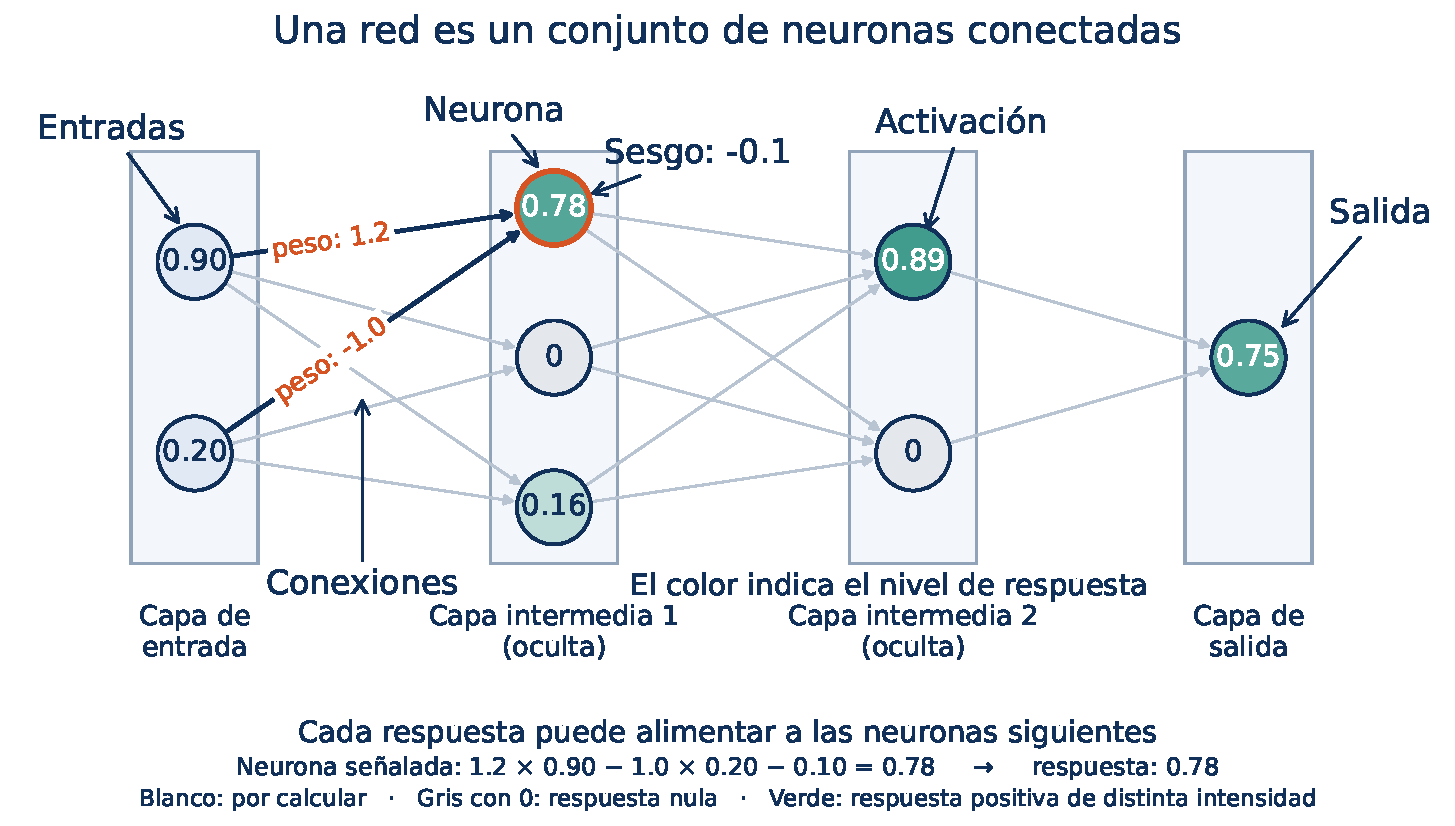
\includegraphics[width=\textwidth,height=4.4cm,keepaspectratio]{red_general.pdf}
    \par\smallskip
    \smallskip
    \href{run:simulacion/propagacion_red.gif}{\small\textbf{Ver el recorrido de las señales en la red}}
    \note{Mostrar primero la forma general de una red, con un ejemplo numérico, antes de la fórmula general y de la analogía con una función matemática: esa formalización viene después. Recorrer las flechas de las etiquetas: entradas, una neurona, conexiones, activación y salida. La activación es la respuesta numérica que una neurona entrega a las siguientes; su color indica intensidad. En el ejemplo hay respuestas cero y respuestas positivas de distintos tamaños, no solo encendido o apagado. Abrir simulacion/propagacion_red.gif: representa tres entradas distintas con parámetros fijos, sin entrenamiento. El blanco con puntos suspensivos significa por calcular; gris con cero es una respuesta calculada y nula. El GIF ordena el cálculo por grupos para explicarlo y no representa el tiempo físico de un cerebro. Retomar la analogía biológica de recibir, integrar y transmitir señales. Los pesos motivan la distinta influencia de las conexiones; aprender implicará ajustarlos más adelante. El sesgo no es una estructura anatómica.}
\end{frame}

\begin{frame}{Historia de las redes neuronales: 1943--1986}
    \begin{center}
        \begin{tikzpicture}[>=Latex,x=1cm,y=1cm,
            evento/.style={anchor=west,align=left,text width=10.7cm,
                inner sep=2.5mm,fill=gray!9,rounded corners=2pt,font=\small}]
            \draw[->,fondo!40,line width=1.1pt] (1.6,0.5) -- (1.6,-4.25);
            \foreach \altura/\fecha in {0/1943,-1.2/1958,-2.4/1969,-3.6/1986} {
                \fill[verde] (1.6,\altura) circle (0.075);
                \node[anchor=east,text=fondo,font=\large\bfseries] at (1.25,\altura) {\fecha};
            }
            \node[evento] at (1.95,0) {\textbf{McCulloch y Pitts}\par
                Proponen un modelo matemático de neurona.};
            \node[evento] at (1.95,-1.2) {\textbf{Rosenblatt}\par
                Desarrolla el perceptrón, un algoritmo de aprendizaje supervisado.};
            \node[evento] at (1.95,-2.4) {\textbf{Minsky y Papert}\par
                Publican \textit{Perceptrons}, destacando las limitaciones del perceptrón.};
            \node[evento] at (1.95,-3.6) {\textbf{Rumelhart, Hinton y Williams}\par
                Difunden el uso de la retropropagación para entrenar redes neuronales.};
        \end{tikzpicture}
    \end{center}

\end{frame}

\begin{frame}{Historia de las redes neuronales: 1989--2017}
    \begin{center}
        \begin{tikzpicture}[>=Latex,x=1cm,y=1cm,
            evento/.style={anchor=west,align=left,text width=10.7cm,
                inner sep=2.5mm,fill=gray!9,rounded corners=2pt,font=\small}]
            \draw[->,fondo!40,line width=1.1pt] (1.6,0.5) -- (1.6,-4.25);
            \foreach \altura/\fecha in {0/1989,-1.2/2010,-2.4/2012,-3.6/2017} {
                \fill[verde] (1.6,\altura) circle (0.075);
                \node[anchor=east,text=fondo,font=\large\bfseries] at (1.25,\altura) {\fecha};
            }
            \node[evento] at (1.95,0) {\textbf{LeCun y sus colegas}\par
                Aplican redes neuronales (LeNet) a clasificar dígitos manuscritos.};
            \node[evento] at (1.95,-1.2) {\textbf{Entrenamiento con GPUs}\par
                Se populariza el uso de GPUs para entrenar redes neuronales.};
            \node[evento] at (1.95,-2.4) {\textbf{Hinton y sus colegas}\par
                Ganan el concurso ImageNet con una red profunda.};
            \node[evento] at (1.95,-3.6) {\textbf{Vaswani et al.}\par
                Introducen el modelo Transformer.};
        \end{tikzpicture}
    \end{center}
    \begin{caja}[yellowbox]
        \small Los avances combinan modelos, algoritmos, datos y capacidad de cómputo.
    \end{caja}
\end{frame}

\begin{frame}{Una función matemática: de la entrada a la salida}
    \begin{columns}[c]
        \begin{column}{0.45\textwidth}
            Una función asigna a cada entrada una única salida.
            \begin{caja}[greenbox]
                \centering
                \textbf{Ejemplo: una regla conocida}
                \[f(x)=2x+1,\qquad y=f(x).\]
                Entrada $1\ \longrightarrow\ f\ \longrightarrow\ $ salida $3$.
            \end{caja}
            \medskip
            \centering
            \begin{tabular}{cc}
                \toprule
                Entrada $x$ & Salida $f(x)$\\
                \midrule
                $-1$ & $-1$\\
                $0$ & $1$\\
                $1$ & $3$\\
                $2$ & $5$\\
                \bottomrule
            \end{tabular}
        \end{column}
        \begin{column}{0.50\textwidth}
            \centering
            \begin{tikzpicture}[x=1.05cm,y=0.48cm,>=Latex,every node/.style={font=\small}]
                \draw[gray!18,step=1] (-2,-3) grid (2,5);
                \draw[->,fondo!70] (-2.4,0)--(2.6,0) node[right] {$x$};
                \draw[->,fondo!70] (0,-3.6)--(0,5.9) node[above] {$y$};
                \foreach \x in {-2,-1,1,2} {
                    \draw (\x,0.09)--(\x,-0.09) node[below] {$\x$};
                }
                \foreach \y in {-3,-1,1,3,5} {
                    \draw (0.05,\y)--(-0.05,\y) node[left] {$\y$};
                }
                \draw[verde,line width=1.3pt] (-2,-3)--(2,5);
                \node[text=verde,anchor=west] at (0.75,5.6) {$y=2x+1$};
                \draw[naranja,dashed] (1,0)--(1,3)--(0,3);
                \fill[naranja] (1,3) circle (2pt);
                \node[anchor=west,text=naranja] at (1.08,3) {$(1,3)$};
            \end{tikzpicture}
        \end{column}
    \end{columns}
    \medskip
    \begin{caja}[yellowbox]
        El gráfico representa los pares \textbf{entrada--salida} que cumplen la regla de la función.
    \end{caja}
    \note{Primero explicar la función matemática, sin hablar todavía de pesos, entrenamiento ni redes. Calcular dos filas de la tabla y ubicarlas en la recta. Una función asigna una única salida a cada entrada, aunque distintas entradas pueden compartir una salida en otras funciones. Aquí la regla se conoce de antemano. En la siguiente diapositiva se introducirá una familia de funciones ajustables que puede aprender a aproximar una relación a partir de ejemplos.}
\end{frame}

% Recrea en TikZ el esquema de la página 10/51 de la presentación de MRI.
% La función se presenta primero a la izquierda; la red aparece a la derecha.
\begin{frame}{Una red neuronal como función ajustable}
    \begin{center}
        \resizebox{0.95\linewidth}{!}{% Recreación vectorial del esquema de DL_MRI_presentation.pdf, p. 10/51.
% La función se motiva a la izquierda y su implementación como red a la derecha.
\begin{tikzpicture}[x=1cm,y=1cm,>=Latex,
    every node/.style={font=\small},
    conexion/.style={draw=fondo!60,line width=0.6pt},
    neurona/.style={circle,draw=fondo,line width=0.8pt,fill=white,minimum size=4mm,inner sep=0pt},
    proceso/.style={draw=fondo,rounded corners=2pt,fill=fondo!7,align=center,inner sep=3mm}]
    \path[use as bounding box] (-0.2,-2.05) rectangle (13.55,1.8);

    % Una función ajustable: entrada y salida en sentido de izquierda a derecha.
    \node[font=\small\bfseries] at (2.5,1.55) {Una función con parámetros};
    \node[draw=verde,text=verde,inner sep=2mm] (entradafuncion) at (0.1,0.45) {$x$};
    \node[proceso,minimum width=15mm,minimum height=12mm] (funcion) at (2.4,0.45) {$f_{\theta}$};
    \node[draw=naranja,text=naranja,inner sep=2mm] (salidafuncion) at (4.85,0.45) {$\hat y=f_{\theta}(x)$};
    \draw[->,conexion] (entradafuncion) -- (funcion);
    \draw[->,conexion] (funcion) -- (salidafuncion);
    \node[below=2mm of entradafuncion,font=\scriptsize] {entrada};
    \node[below=2mm of salidafuncion,font=\scriptsize] {predicción};
    \node[proceso,fill=verde!9,draw=verde!55,text width=47mm,font=\small] (ajuste) at (2.5,-1.3)
        {Ajustar los parámetros $\theta$ con ejemplos $(x,y)$ para que la predicción se aproxime a $y$.};
    \draw[->,verde] (ajuste.north) -- (funcion.south);

    % Una red realiza esa función. Se distinguen parámetros y valores predichos.
    \draw[fondo!15] (6.15,-1.9) -- (6.15,1.75);
    \node[font=\small\bfseries] at (9.7,1.55) {Una red implementa esa función};
    \node[neurona,fill=verde!20,draw=verde] (entrada) at (7.0,0.35) {};
    \foreach \i/\altura in {1/1.0,2/0.35,3/-0.3} {
        \node[neurona] (a\i) at (8.5,\altura) {};
        \node[neurona] (b\i) at (10.0,\altura) {};
        \draw[conexion] (entrada) -- (a\i);
    }
    \foreach \i in {1,2,3} {
        \foreach \j in {1,2,3} {
            \draw[conexion] (a\i) -- (b\j);
        }
    }
    \node[neurona,fill=naranja!25,draw=naranja] (salida) at (11.5,0.35) {};
    \foreach \i in {1,2,3} {\draw[conexion] (b\i) -- (salida);}
    \node[above=2mm of entrada,text=verde,font=\scriptsize] {entrada $x$};
    \node[above=2mm of salida,text=naranja,font=\scriptsize] {predicción $\hat y$};
    \node[proceso,text width=29mm,font=\scriptsize] (optimizar) at (8.15,-1.4)
        {Entrenamiento\\actualizar parámetros};
    \node[proceso,draw=naranja,fill=naranja!8,text width=21mm,font=\scriptsize] (perdida) at (11.85,-1.4)
        {Función de pérdida};
    \draw[->,conexion] (salida.south) -- (perdida.north);
    \node[text=verde,font=\scriptsize,align=center] (referencia) at (13.0,-0.65) {referencia\\$y$};
    \draw[->,verde] (referencia.south) -- ++(0.5,0) |- (perdida.east);
    \draw[->,conexion] (perdida.west) -- (optimizar.east);
    \draw[->,conexion] (optimizar.north) -- (a3.south);
\end{tikzpicture}
}
    \end{center}
    \begin{caja}[orangebox]
        \begin{itemize}
            \item Una \tcg{red neuronal} aprende una relación entre \tcg{entrada} y \tcg{salida} ajustando sus parámetros internos.
            \item El entrenamiento busca minimizar una \tcr{función de pérdida}, midiendo el error entre la salida y la referencia.
            \item Mediante la \tcg{optimización}, se actualizan los parámetros para reducir ese error.
        \end{itemize}
    \end{caja}
    \note{Esquema recreado en TikZ a partir de DL_MRI_presentation.pdf, página 10/51, con la función a la izquierda. Empezar por entrada, función ajustable y salida; pasar a la red que implementa la función. La predicción se compara con una referencia y la pérdida guía el ajuste. Theta agrupa los parámetros; para la neurona lineal serán pesos y sesgo. La referencia se utiliza para entrenar o evaluar, no se necesita para producir una predicción después del entrenamiento.}
\end{frame}

\section{Modelos con una neurona o más neuronas}

\begin{frame}{1. Una relación lineal: una neurona}
    \begin{columns}[c]
        \begin{column}{0.25\textwidth}
            \centering\small
            \textbf{Datos de entrenamiento}\par\smallskip
            \begin{tabular}{rr}
                \toprule
                Entrada $x$ & Salida $y$\\
                \midrule
                $-2$ & $-3$\\
                $-1$ & $-1$\\
                $0$ & $1$\\
                $1$ & $3$\\
                $2$ & $5$\\
                \bottomrule
            \end{tabular}
            \par\smallskip{\scriptsize Muestra: 5 de los 21 pares.}
        \end{column}
        \begin{column}{0.72\textwidth}
            \centering
            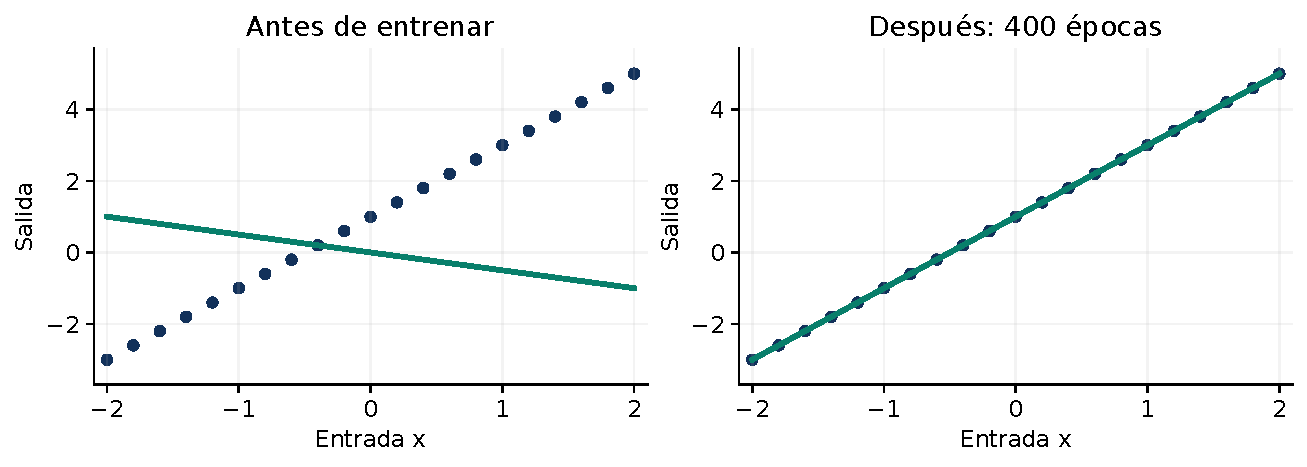
\includegraphics[width=\linewidth,height=2.8cm,keepaspectratio]{simulacion_lineal.pdf}
        \end{column}
    \end{columns}
    \par\medskip
    \begin{columns}[c]
        \begin{column}{0.55\textwidth}
            \begin{caja}[greenbox]
                \textbf{Una entrada, una salida:}\par\smallskip
                \[\hat y=\underbrace{w}_{\text{pendiente}}\,x+
                \underbrace{b}_{\text{desplazamiento}}.\]
                El entrenamiento ajusta dos parámetros.
            \end{caja}
        \end{column}
        \begin{column}{0.40\textwidth}
            \centering
            \begin{tikzpicture}[>=Latex,every node/.style={font=\small},
                neurona/.style={draw=fondo,circle,fill=verde!10,minimum size=8mm}]
                \node (x) at (0,0) {$x$};
                \node[neurona] (suma) at (1.7,0) {$\Sigma$};
                \node (y) at (3.5,0) {$\hat y$};
                \node (b) at (1.7,-0.9) {$b$};
                \draw[->] (x)--node[above] {$w$} (suma);
                \draw[->] (b)--(suma); \draw[->] (suma)--(y);
            \end{tikzpicture}
            \par\smallskip\raggedright\small
            Datos de referencia: $y=2x+1$.\par\smallskip
            Después de entrenar: $w\approx2$, $b\approx1$.\par\smallskip
            Nueva entrada: $1.5\mapsto\hat y\approx4$.
        \end{column}
    \end{columns}
    \medskip
    \href{run:simulacion/simulacion_progresiva.html}{\textbf{Abrir la simulación progresiva}}
    \note{Primera etapa de simulacion/simulacion_progresiva.html. La tabla presenta cinco pares reales del conjunto sintético de 21 observaciones: x se distribuye uniformemente entre -2 y 2 e y=2x+1. Son referencias conocidas que se proporcionan durante el entrenamiento, no predicciones del modelo. Localizar las filas en los puntos del gráfico. Preguntar qué cambia al modificar pendiente y desplazamiento. Reproducir la trayectoria de una neurona de activación identidad: tasa 0.05 y 400 épocas. La entrada 1.5 no aparece en los datos de entrenamiento y se consulta después. El modelo aprende aproximadamente 2 y 1 como peso y sesgo. En terminología estricta, al incluir el sesgo la función es afín; se mantiene lineal por su uso habitual en regresión.}
\end{frame}

\begin{frame}{2. Dos variables explican una salida}
    \textbf{Ejemplo: gasto mensual en alimentación de un hogar.}\par\medskip
    \begin{columns}[T]
        \begin{column}{0.48\textwidth}
            \small
            $x_1$: ingreso mensual, en \textbf{miles de u.m.}\par\smallskip
            $x_2$: número de integrantes.\par\smallskip
            $y$: gasto mensual, en \textbf{u.m.}\par\medskip
            \centering
            \begin{tabular}{rrrr}
                \toprule
                Hogar & $x_1$ & $x_2$ & $y$\\
                \midrule
                1 & 1.0 & 1 & 150\\
                3 & 1.0 & 3 & 230\\
                7 & 1.5 & 2 & 220\\
                14 & 2.0 & 4 & 330\\
                18 & 3.0 & 3 & 350\\
                25 & 4.0 & 5 & 490\\
                \bottomrule
            \end{tabular}
            \par\smallskip
            {\scriptsize Se muestran 6 de las 25 observaciones sintéticas.}
        \end{column}
        \begin{column}{0.48\textwidth}
            \centering
            \begin{tikzpicture}[>=Latex,every node/.style={font=\small},
                neurona/.style={draw=fondo,circle,fill=verde!10,minimum size=8mm}]
                \node (x1) at (0,0.75) {$x_1$};
                \node (x2) at (0,-0.75) {$x_2$};
                \node[neurona] (suma) at (2.0,0) {$\Sigma$};
                \node (y) at (4.0,0) {$\hat y$};
                \node (b) at (2.0,-1.1) {$b$};
                \draw[->] (x1)--node[above,sloped] {$w_1$} (suma);
                \draw[->] (x2)--node[below,sloped] {$w_2$} (suma);
                \draw[->] (b)--(suma); \draw[->] (suma)--(y);
            \end{tikzpicture}
            \par\smallskip
            \begin{caja}[greenbox]
                \centering
                \textbf{Una neurona, tres parámetros:}\par\smallskip
                {\large $\hat y=w_1x_1+w_2x_2+b.$}\par\smallskip
                \small Estimamos $w_1$, $w_2$ y $b$ con los datos.
            \end{caja}
            \par\smallskip\small
            Después de entrenar:\par\smallskip
            $w_1\approx60,\quad w_2\approx40,\quad b\approx50$.
        \end{column}
    \end{columns}
    \medskip
    \begin{caja}[yellowbox]
        \small Hogar nuevo: ingreso $2500$ u.m., $3$ integrantes $\Rightarrow$
        $\hat y=60(2.5)+40(3)+50\approx320$ u.m.
    \end{caja}
    \note{Segunda etapa de simulacion/simulacion_progresiva.html, también disponible en simulacion/simulacion_multivariable.html. Es regresión lineal múltiple: una variable respuesta depende de dos variables explicativas. Se estiman los parámetros; se predice el gasto. Hay una sola neurona con dos pesos y un sesgo. Los 25 hogares son datos sintéticos sin ruido, generados con y=60x1+40x2+50. Los identificadores de la tabla corresponden a las filas del CSV completo. El ingreso se expresa en miles: 2500 u.m. se introduce como 2.5; el gasto conserva unidades monetarias. El hogar (2.5,3) no se usa para entrenar. Comparar hogares con el mismo ingreso y distinto número de integrantes para motivar w2; mantener integrantes y variar ingreso para motivar w1. Las asociaciones del ejemplo no demuestran causalidad ni describen una economía real.}
\end{frame}

\begin{frame}{Entre capas: composición de funciones}
    \centering
    \begin{tikzpicture}[>=Latex,every node/.style={font=\small},
        capa/.style={draw=fondo,rounded corners,fill=verde!10,minimum width=23mm,minimum height=10mm}]
        \node (x) at (0,0) {$x$};
        \node[capa] (f1) at (2,0) {$f_1$};
        \node (h) at (4,0) {$h=f_1(x)$};
        \node[capa] (f2) at (6.2,0) {$f_2$};
        \node (y) at (8.6,0) {$\hat y=f_2(h)$};
        \draw[->] (x)--(f1); \draw[->] (f1)--(h);
        \draw[->] (h)--(f2); \draw[->] (f2)--(y);
    \end{tikzpicture}
    \par\medskip
    {\small Con activación identidad:
    $f_1(x)=w_1x+b_1$ y $f_2(h)=w_2h+b_2$.}\par
    \begin{align*}
        \hat y &=(f_2\circ f_1)(x)=f_2(f_1(x))\\
               &=w_2(w_1x+b_1)+b_2\\
               &=\underbrace{(w_2w_1)}_{A}\,x+
                 \underbrace{(w_2b_1+b_2)}_{B}.
    \end{align*}
    \begin{caja}[orangebox]
        \textbf{Componer funciones afines sigue dando una función afín:} $\hat y=Ax+B$.
    \end{caja}
    \smallskip
    \begin{caja}[yellowbox]
        \small Para representar relaciones curvas, introduciremos \textbf{activaciones no lineales}.
    \end{caja}
    \smallskip\scriptsize Dentro de una neurona se suman entradas ponderadas; entre capas se componen funciones.
    \note{Distinguir explícitamente dos niveles: cada neurona combina sus entradas mediante una suma ponderada y un sesgo; la salida de una capa alimenta a la siguiente y eso es composición. El ejemplo escalar usa una neurona por capa para mostrar la composición sin notación matricial. El argumento también vale para capas de varias neuronas: F2(F1(x))=A2(A1x+b1)+b2 sigue siendo afín si todas las activaciones son identidad. La expresión anterior con v1h1+v2h2+c era la combinación dentro de la neurona de salida, pero no explicitaba suficientemente la composición de capas. Se asume que no se añaden características no lineales a la entrada.}
\end{frame}

\begin{frame}{3. ¿Puede una recta aprender el cuadrado?}
    \begin{columns}[c]
        \begin{column}{0.26\textwidth}
            \centering\small
            \textbf{Función cuadrática}\par\medskip
            \begin{tabular}{rr}
                \toprule
                Entrada $x$ & Salida $y$\\
                \midrule
                $-2$ & $4$\\
                $-1$ & $1$\\
                $0$ & $0$\\
                $1$ & $1$\\
                $2$ & $4$\\
                \bottomrule
            \end{tabular}
            \par\medskip $y=x^2$\par\smallskip
            \scriptsize Muestra de los 21 pares de entrenamiento.
        \end{column}
        \begin{column}{0.70\textwidth}
            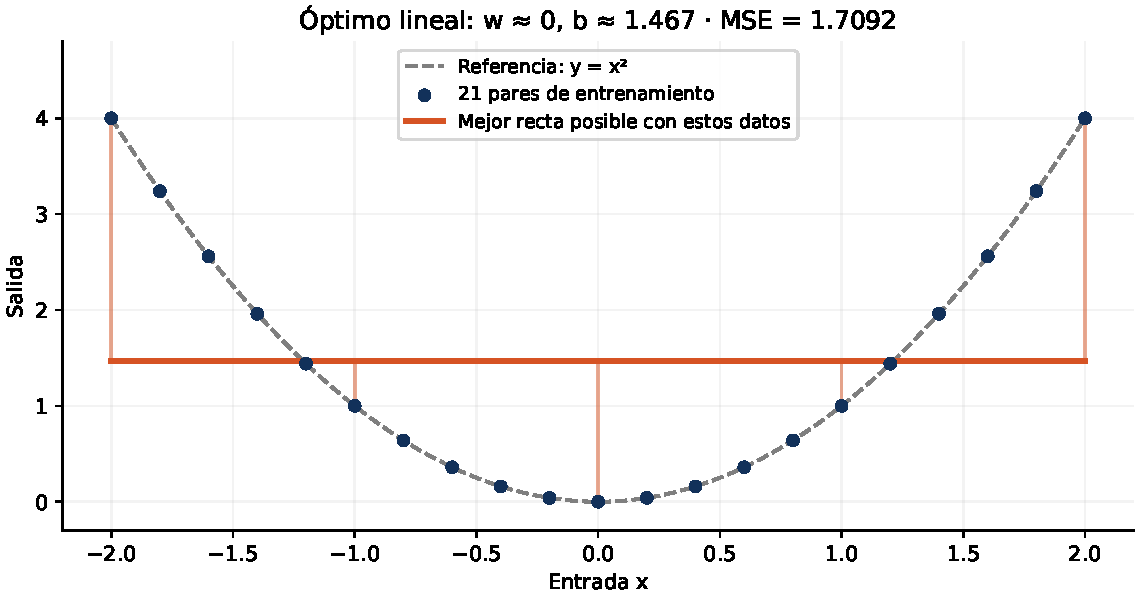
\includegraphics[width=\linewidth,height=4.3cm,keepaspectratio]{limite_lineal_cuadrado.pdf}
        \end{column}
    \end{columns}
    \medskip
    \begin{caja}[orangebox]
        \textbf{Ajustar mejor los parámetros no cambia la forma del modelo.}\par\smallskip
        $\hat y=wx+b$ sigue siendo una recta; no reproduce la curvatura de $x^2$.
    \end{caja}
    \smallskip\small Necesitamos ampliar la familia de funciones: el siguiente ejemplo incorpora activaciones no lineales.
    \note{La recta naranja es el mejor ajuste por mínimos cuadrados a los 21 pares, no una mala inicialización. Por simetría, su pendiente es cero y el sesgo es el promedio de los cuadrados. Incluso el óptimo deja residuos: añadir épocas no elimina ese límite. Una recta puede aproximar localmente una curva, pero no reproducir x al cuadrado en todo este intervalo. Se considera x como única característica: añadir x al cuadrado como característica sería cambiar la representación. La siguiente diapositiva conserva la simulación de la red no lineal.}
\end{frame}


\begin{frame}{Simulación: ¿qué cambia cuando la red aprende?}
    % Valores obtenidos del entrenamiento, generados autom?ticamente.
\newcommand{\prediccionCuadrado}{2.307}
\newcommand{\mseCuadrado}{0.0032}

    \centering
    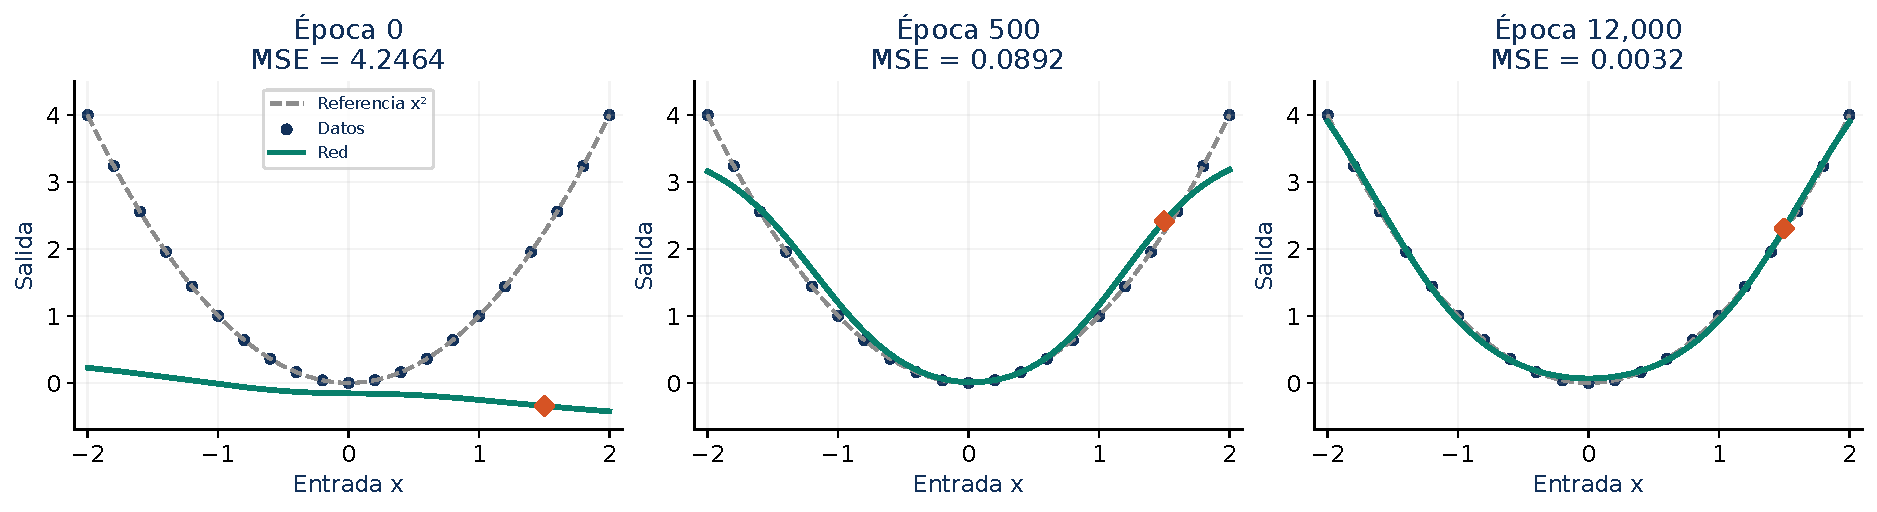
\includegraphics[width=0.97\textwidth,height=3.5cm,keepaspectratio]{simulacion_cuadrado.pdf}
    \par\smallskip
    \begin{columns}[c]
        \begin{column}{0.59\textwidth}
            \begin{caja}[greenbox]
                \textbf{Dentro de cada neurona:}\par\smallskip
                \[z_j=\underbrace{w_j}_{\text{peso}}\,\underbrace{x}_{\text{entrada}}+
                \underbrace{b_j}_{\text{sesgo}},\qquad a_j=\tanh(z_j).\]
            \end{caja}
        \end{column}
        \begin{column}{0.37\textwidth}
            \raggedright
            \textbf{Una entrada no usada al entrenar:}\par\smallskip
            $x=1.5\ \Rightarrow\ \hat y\approx\prediccionCuadrado$.\par\smallskip
            Referencia: $1.5^2=2.25$.
        \end{column}
    \end{columns}
    \medskip
    \href{run:simulacion/simulacion_cuadrado.html}{\textbf{Abrir simulación interactiva: pesos, sesgos y predicciones}}
    \par\smallskip
    {\scriptsize Red 1--6--1 con tanh, 21 pares, semilla 7 y descenso por gradiente. El punto naranja consulta $x=1.5$.}
    \note{Usar la etapa 3 de simulacion/simulacion_progresiva.html o la demostración original simulacion/simulacion_cuadrado.html. Funcionan sin internet. Los estados proceden de un entrenamiento real. Mostrar inicio, 500 y 12000 épocas, y seguir el cálculo z=wx+b seguido de tanh en una neurona. La salida combina las seis respuestas con pesos v y su propio sesgo c. Cambiar la entrada después de entrenar mantiene los parámetros fijos. Comparar con la neurona lineal. Cerrar la progresión: una entrada afín usa un peso y un sesgo; dos entradas afines usan dos pesos y un sesgo en la misma neurona; una relación curva motiva no linealidad. Una función con detalles más variados puede necesitar más capacidad, pero no hay una regla universal que asigne un tamaño de red a cada complejidad. El GIF conserva la animación cuadrática y el PDF muestra tres estados estáticos.}
\end{frame}

\section{Construir el modelo: combinación y activación}

\begin{frame}{Una neurona: entradas, pesos, sesgo y salida}
    \centering
    \begin{tikzpicture}[scale=0.82,transform shape,>=Latex, every node/.style={font=\small},
        entrada/.style={circle,draw=fondo,minimum size=8mm},
        operacion/.style={draw=fondo,rounded corners,fill=fondo!5,minimum height=12mm}]
        \node[entrada] (x1) at (0,1.1) {$x_1$};
        \node at (0,0) {$\vdots$};
        \node[entrada] (xd) at (0,-1.1) {$x_d$};
        \node[operacion,minimum width=25mm] (sum) at (3.2,0) {$z=\sum_j w_jx_j+b$};
        \node[operacion,minimum width=18mm] (act) at (6.4,0) {$\sigma(z)$};
        \node (out) at (8.5,0) {$\hat y$};
        \node[draw=verde,rounded corners] (bias) at (3.2,1.6) {sesgo $b$};
        \draw[->] (x1) -- node[above,sloped] {$w_1$} (sum);
        \draw[->] (xd) -- node[below,sloped] {$w_d$} (sum);
        \draw[->,verde] (bias) -- (sum);
        \node[below=3mm of sum] {combinación};
        \node[below=3mm of act] {activación};
        \draw[->] (sum) -- (act);
        \draw[->] (act) -- node[above] {salida} (out);
    \end{tikzpicture}
    \par\smallskip
    \begin{columns}[c]
        \begin{column}{0.33\textwidth}
            \centering\small
            \textbf{Vectores columna}
            \[\bm x=\begin{pmatrix}x_1\\\vdots\\x_d\end{pmatrix},\qquad
              \bm w=\begin{pmatrix}w_1\\\vdots\\w_d\end{pmatrix}.\]
        \end{column}
        \begin{column}{0.63\textwidth}
            \centering\small
            \textbf{La suma ponderada es un producto interno}
            \[\bm w^{\top}\bm x=
              \begin{pmatrix}w_1&\cdots&w_d\end{pmatrix}
              \begin{pmatrix}x_1\\\vdots\\x_d\end{pmatrix}
              =\sum_{j=1}^d w_jx_j.\]
            $z=\bm w^{\top}\bm x+b,\qquad\hat y=\sigma(\bm w^{\top}\bm x+b).$
        \end{column}
    \end{columns}
    \smallskip
    \begin{caja}[greenbox]
        \small $\bm x,\bm w\in\R^d$, $b\in\R$; $\bm w^{\top}\bm x$ es un escalar.\quad
        \textbf{Parámetros entrenables:} $d$ pesos y un sesgo, es decir, $d+1$.
    \end{caja}
    \note{Presentar x y w como vectores columna de tamaño d por 1. La transposición convierte w en una fila de tamaño 1 por d; al multiplicarla por x se obtiene un escalar, equivalente a la suma ponderada del esquema. El sesgo se añade después del producto interno. No confundir el producto interno con el producto elemento a elemento. Los componentes de x son características de una observación; los pesos y el sesgo son parámetros entrenables.}
\end{frame}


\begin{frame}{La activación transforma la combinación}
    \centering
    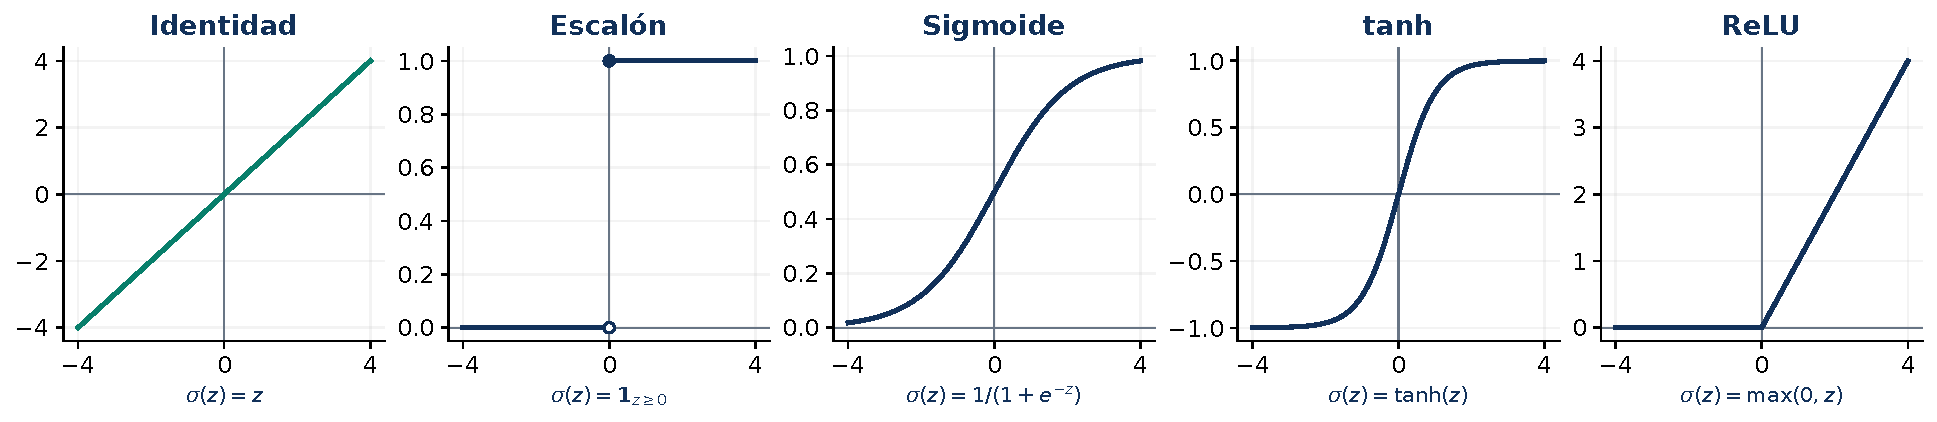
\includegraphics[width=\textwidth,height=2.3cm,keepaspectratio]{activaciones.pdf}
    \par\smallskip
    {\small
    \renewcommand{\arraystretch}{1.15}
    \begin{tabular}{@{}p{0.13\textwidth}p{0.43\textwidth}p{0.37\textwidth}@{}}
        \toprule
        \textbf{Activación} & \textbf{¿Dónde y para qué?} & \textbf{Ejemplo de tarea} \\
        \midrule
        Identidad & Salida continua en regresión. & Predecir un precio o consumo. \\
        Escalón & Salida binaria del perceptrón clásico. & Separar dos clases con un umbral. \\
        Sigmoide & Salida entre 0 y 1 en clasificación binaria. & Estimar si un correo es spam. \\
        $\tanh$ & Capas ocultas: representar relaciones no lineales. & Aproximar $x^2$, como en la simulación. \\
        ReLU & Capas ocultas de redes profundas. & Aprender patrones para clasificar imágenes. \\
        \bottomrule
    \end{tabular}
    }
    \par\smallskip
    \note{Son usos habituales, no una correspondencia exclusiva entre activación y tarea. Hoy usamos identidad para regresión. El escalón da una decisión dura y no se usa con el descenso de gradiente habitual. La sigmoide puede interpretarse como probabilidad de una clase cuando el modelo se entrena para clasificación binaria con una pérdida adecuada, como entropía cruzada binaria; su rango por sí solo no garantiza esa interpretación. Tanh también se usa en estados de redes recurrentes. ReLU es habitual en capas ocultas de redes densas y convolucionales; la activación final depende de la tarea.}
\end{frame}

\begin{frame}{¿Qué significa ``perceptrón lineal'' en esta clase?}
    \begin{columns}[T]
        \begin{column}{0.48\textwidth}
            \begin{caja}
                \textbf{Perceptrón clásico}\par\medskip
                \[\hat y=\mathbf{1}_{\{\bm w^\top\bm x+b\geq0\}}\]
                Activación escalón.\par\smallskip
                Se utiliza para clasificación binaria.
            \end{caja}
        \end{column}
        \begin{column}{0.48\textwidth}
            \begin{caja}[greenbox]
                \textbf{Neurona para regresión}\par\medskip
                \[\hat y=\bm w^\top\bm x+b\]
                Activación identidad.\par\smallskip
                Es el modelo del notebook de hoy.
            \end{caja}
        \end{column}
    \end{columns}
    \vspace{5mm}
    \note{La distinción evita mezclar la regla clásica del perceptrón con descenso de gradiente de MSE. Para esta clase todos los gradientes y las aplicaciones corresponden a la columna derecha.}
\end{frame}

\section{Aprender: medir el error y actualizar parámetros}

\begin{frame}{¿Qué significa aprender a partir de ejemplos?}
    \[\mathcal D=\{(\bm x^{(i)},y^{(i)})\}_{i=1}^{N},\qquad
      \hat y^{(i)}=\bm w^\top\bm x^{(i)}+b.\]
    \vspace{1mm}
    \begin{center}
        \begin{tikzpicture}[>=Latex,node distance=5mm,
            paso/.style={draw=fondo,rounded corners,fill=fondo!5,align=center,
                minimum height=12mm,text width=18mm,inner sep=2mm,font=\small}]
            \node[paso] (datos) {Datos\\$(\bm x,y)$};
            \node[paso,right=of datos] (modelo) {Modelo\\$\hat y$};
            \node[paso,right=of modelo] (loss) {Pérdida\\$\mathcal L$};
            \node[paso,right=of loss] (grad) {Gradiente\\$\nabla\mathcal L$};
            \node[paso,right=of grad] (update) {Actualizar\\$\bm w,b$};
            \draw[->] (datos)--(modelo);
            \draw[->] (modelo)--(loss);
            \draw[->] (loss)--(grad);
            \draw[->] (grad)--(update);
            \draw[->,verde] (update.south)--++(0,-0.6)-|(modelo.south);
        \end{tikzpicture}
    \end{center}
    \vspace{4mm}
    \begin{caja}[greenbox]
        \textbf{Entrenamiento:} ajustar los parámetros para reducir la pérdida sobre los ejemplos disponibles.
    \end{caja}
    \note{Las etiquetas y las entradas permanecen fijas en este experimento; cambiamos parámetros. Aclarar que disminuir pérdida de entrenamiento no prueba generalización a datos nuevos.}
\end{frame}

\begin{frame}{Una pérdida para regresión: error cuadrático medio}
    \begin{columns}[c]
        \begin{column}{0.53\textwidth}
            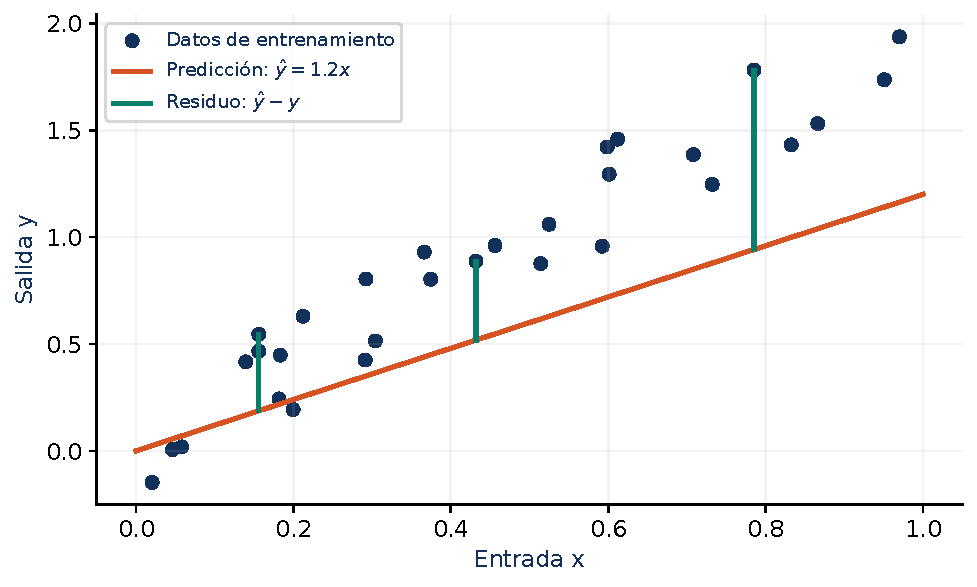
\includegraphics[width=\linewidth]{residuos.pdf}
        \end{column}
        \begin{column}{0.44\textwidth}
            \begin{caja}
                \textbf{Residuo de una observación}
                \[e_i=\hat y^{(i)}-y^{(i)}.\]
                \textbf{Promedio de los errores al cuadrado}
                \[\mathcal L(\bm w,b)=\frac1N\sum_{i=1}^N e_i^2.\]
            \end{caja}
            \medskip
            \small El cuadrado evita cancelaciones y penaliza errores grandes.
        \end{column}
    \end{columns}
    \note{Preguntar por qué no basta con promediar residuos con signo. La figura usa los datos del Ejemplo 1 y una recta ilustrativa de pendiente 1.2.}
\end{frame}

\begin{frame}{Recordatorio: el gradiente señala la mayor subida}
    {\small Ejemplo con dos parámetros:
    $\mathcal L(w,b)=2(w-2)^2+(b+1)^2$, con mínimo en $(w,b)=(2,-1)$.}
    \par\smallskip
    \centering
    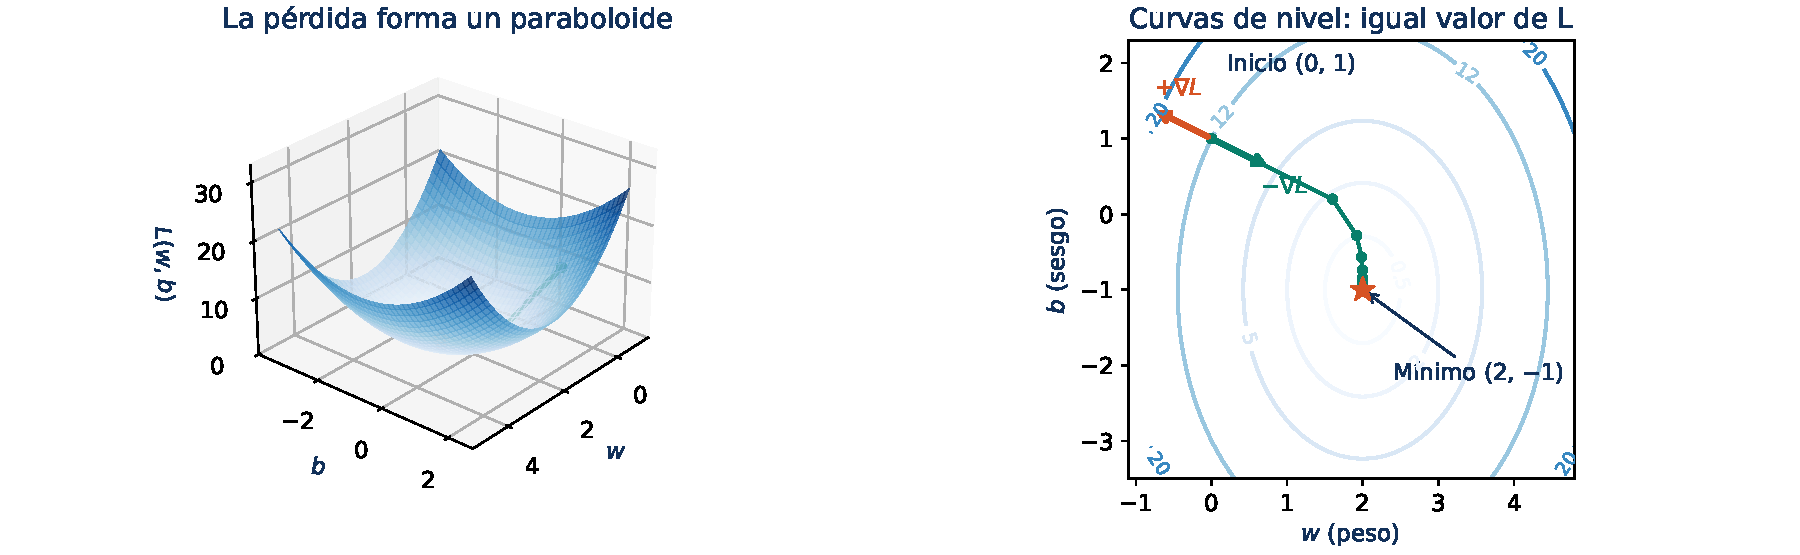
\includegraphics[width=\textwidth,height=3.65cm,keepaspectratio]{gradiente_paraboloide.pdf}
    \par
    {\small
    $\displaystyle\nabla\mathcal L=
    \begin{pmatrix}\partial_w\mathcal L\\\partial_b\mathcal L\end{pmatrix}
    =\begin{pmatrix}4(w-2)\\2(b+1)\end{pmatrix}.$
    \quad En $(0,1)$: $\nabla\mathcal L=(-8,4)^\top$.}
    \par\smallskip
    \begin{caja}[greenbox]
        \small\raggedright
        $+\nabla\mathcal L$: mayor crecimiento local.
        $-\nabla\mathcal L$: mayor descenso local.\par\smallskip
        Con $\eta=0.2$: $(0,1)-0.2(-8,4)=(1.6,0.2)$;
        la pérdida baja de $12$ a $1.76$. Repetimos para acercarnos al mínimo.
    \end{caja}
    \note{Cada punto del plano representa una elección de peso y sesgo, no una observación de los datos. La altura representa la pérdida. Las curvas unen parámetros con igual pérdida; el gradiente es perpendicular a ellas y apunta hacia valores mayores. Las flechas se escalan para facilitar la lectura; los puntos verdes usan pasos reales con eta=0.2. Esta pérdida es exactamente el MSE de dos datos sintéticos: x=+-sqrt(2), y=2x-1. El gradiente indica el mayor crecimiento local por unidad de distancia en la norma euclídea; su opuesto es una dirección de descenso si el gradiente no es cero y el paso es suficientemente pequeño. No apunta necesariamente en línea recta al mínimo. En este paraboloide convexo, con la tasa elegida, los pasos convergen al mínimo global; en una red no lineal no hay esa garantía general.}
\end{frame}

\begin{frame}{¿Cómo sabemos hacia dónde cambiar el modelo?}
    Para una entrada, $\hat y^{(i)}=wx^{(i)}+b$ y $\sigma'(z)=1$:
    \begin{align*}
        \frac{\partial\mathcal L}{\partial w}
            &=\frac{2}{N}\sum_{i=1}^N
              \underbrace{(\hat y^{(i)}-y^{(i)})}_{\text{error}}
              \underbrace{x^{(i)}}_{\partial\hat y^{(i)}/\partial w},\\[3mm]
        \frac{\partial\mathcal L}{\partial b}
            &=\frac{2}{N}\sum_{i=1}^N
              (\hat y^{(i)}-y^{(i)})\underbrace{1}_{\partial\hat y^{(i)}/\partial b}.
    \end{align*}
    \begin{caja}[orangebox]
        \textbf{El sesgo también aprende si forma parte del modelo.}\par\smallskip
        En el Ejemplo 1 se fija $b=0$ y solo se entrena $w$.
    \end{caja}
    \note{Derivar en pizarra un término con la regla de la cadena. Resumen12.pdf, p. 2, muestra un factor cero en la derivada respecto de b: corregirlo para el modelo wx+b. En el notebook del Ejemplo 1, b no participa en la predicción. Para d entradas sustituir x por el vector de características.}
\end{frame}

\begin{frame}{Descenso por gradiente: un paso calculado a mano}
    \begin{caja}[greenbox]
        \centering
        $w_{t+1}=w_t-\eta\,\partial_w\mathcal L,\qquad
        b_{t+1}=b_t-\eta\,\partial_b\mathcal L.$
    \end{caja}
    \vspace{2mm}
    Un dato: $x=2$, $y=5$. Inicio: $w=1$, $b=0$, tasa $\eta=0.1$.
    \begin{align*}
        \hat y&=2, & e&=2-5=-3, & \mathcal L&=9,\\
        \partial_w\mathcal L&=2(-3)(2)=-12,
        & \partial_b\mathcal L&=2(-3)=-6,\\
        w_{\mathrm{nuevo}}&=2.2, & b_{\mathrm{nuevo}}&=0.6,
        & \hat y_{\mathrm{nueva}}&=5.
    \end{align*}
    \actividad{Comprueba el signo}{¿Por qué restar un gradiente negativo aumenta el parámetro?}
    \note{La predicción nueva da pérdida cero solo en este ejemplo de un dato y con esta tasa. No generalizar a otros datos ni afirmar que un paso siempre mejora la pérdida. Ambos gradientes se calculan antes de actualizar.}
\end{frame}

\begin{frame}{La tasa de aprendizaje controla el tamaño del paso}
    \centering
    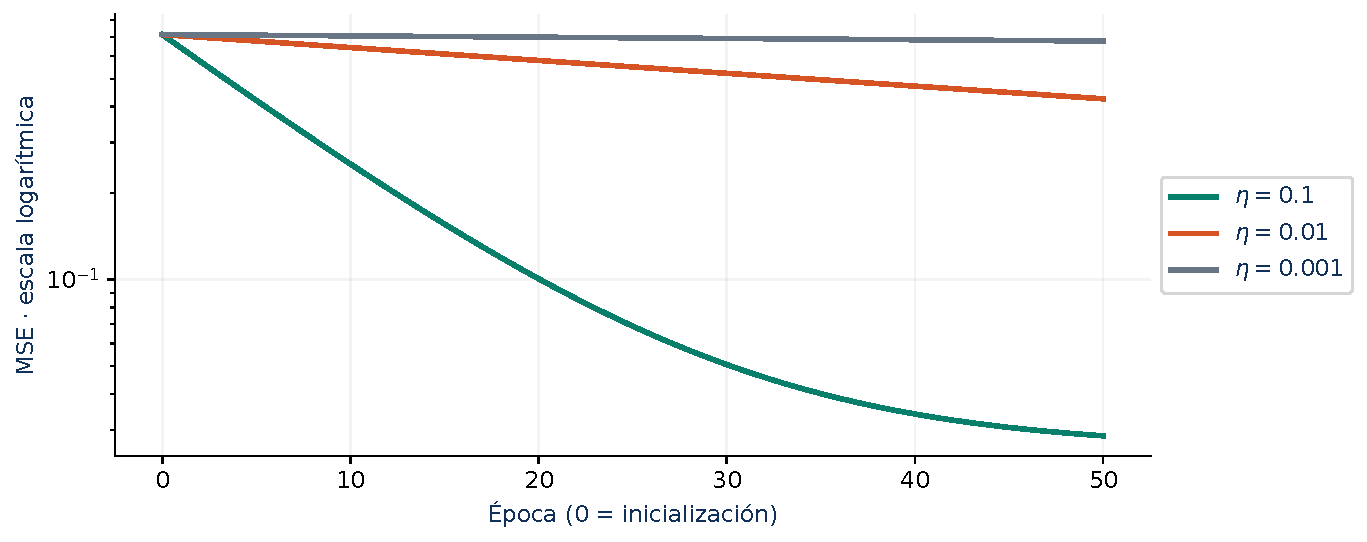
\includegraphics[width=0.83\textwidth,height=4.1cm,keepaspectratio]{tasas_aprendizaje.pdf}
    \begin{caja}[yellowbox]
        \raggedright
        \textbf{Mismos datos, misma inicialización, distinta $\eta$.}\par\smallskip
        Comparamos $\eta=0.1$, $0.01$ y $0.001$: con las mismas 50 épocas, una tasa menor avanza más lentamente en este ejemplo.
    \end{caja}
    \note{Curvas del Ejemplo 1, b=0, 50 épocas; MSE calculado después de cada actualización. Preguntar qué curva elegirían y qué observarían para decidir. Las tasas no son universales: dependen de la escala de los datos y del objetivo.}
\end{frame}

\begin{frame}{Época, lote y actualización: tres ideas distintas}
    \begin{caja}
        \textbf{Época (\textit{epoch}):} un recorrido completo de los datos de entrenamiento.\par\medskip
        \textbf{Lote (\textit{batch}):} subconjunto de observaciones usado para calcular un gradiente.
        Su tamaño, $B$, se llama \textbf{\textit{batch size}}.\par\medskip
        \textbf{Actualización (\textit{update} o \textit{training step}):} un paso que modifica los pesos y el sesgo entrenables usando el gradiente de un lote y la tasa de aprendizaje.
    \end{caja}
    \vspace{3mm}
    \centering
    Para $N=30$ observaciones, sin descartar el último lote:
    \medskip

    \begin{tabular}{lcc}
        \toprule
        Modalidad & Tamaño del lote ($B$) & Actualizaciones por época\\
        \midrule
        Lote completo & 30 & 1\\
        Minilotes & 10 & 3\\
        Una observación por paso & 1 & 30\\
        \bottomrule
    \end{tabular}
    \note{En general hay ceil(N/B) actualizaciones por época si se incluye el último lote incompleto. Resumen12.pdf equipara actualización y época; eso solo coincide en el caso de lote completo del notebook. El bloque final no baraja observaciones.}
\end{frame}

\section{Del modelo al notebook: predecir, ejecutar, explicar}

\begin{frame}[fragile]{Cuatro funciones conectan la teoría con Python}
    \begin{columns}[T]
        \begin{column}{0.50\textwidth}
\begin{lstlisting}
def a(X, w, b):
    return w * X + b

def s(z):
    return z

def L(y_hat, y):
    return ((y_hat - y)**2).mean()

def grad_L(y_hat, y, X):
    error = y_hat - y
    return (2 * np.mean(error * X),
            2 * np.mean(error))
\end{lstlisting}
        \end{column}
        \begin{column}{0.46\textwidth}
            \begin{caja}[greenbox]
                \texttt{a}: combinación.\par\medskip
                \texttt{s}: activación.\par\medskip
                \texttt{L}: pérdida.\par\medskip
                \texttt{grad\_L}: derivadas.\par\medskip
                \texttt{fit}: repite las actualizaciones.
            \end{caja}
            \medskip\small Este código corresponde al \textbf{Ejemplo 2}, con sesgo entrenable.
        \end{column}
    \end{columns}
    \note{Abrir 12-Perceptron-Lineal.ipynb. Identificar funciones antes de ejecutar. En el Ejemplo 1 a devuelve w*X y dLdb es cero: no copiar el sesgo del Ejemplo 2 a ese bloque sin explicar el cambio de modelo.}
\end{frame}

\begin{frame}{Ejemplo 1: una recta que pasa por el origen}
    \[y=2x+\varepsilon,\qquad\hat y=wx,\qquad b=0.\]
    \centering
    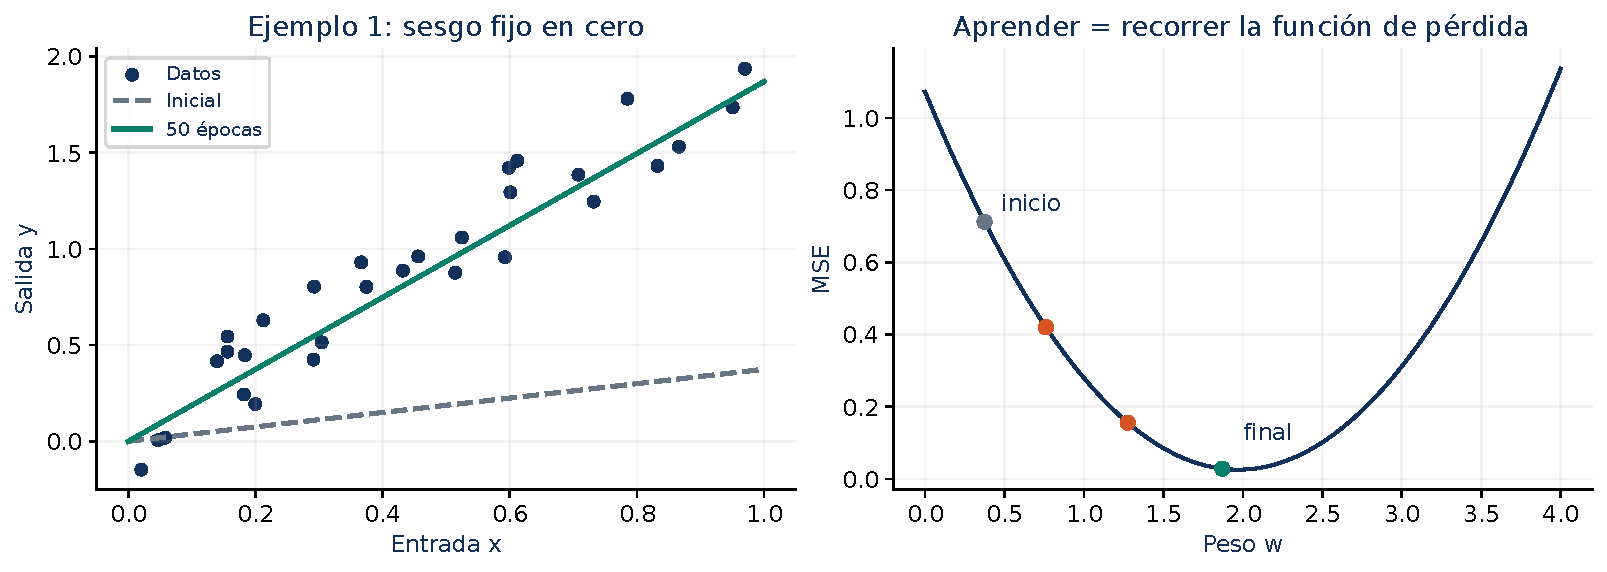
\includegraphics[width=0.92\textwidth,height=4cm,keepaspectratio]{ejemplo_1.pdf}
    \actividad{Antes de ejecutar}{¿Hacia qué valor debería moverse $w$? ¿Esperas que el error final sea exactamente cero?}
    \note{Notebook: Ejemplo 1, celdas 7 a 18 (numeración posicional desde 1). Ejecutar secuencialmente. Datos con ruido: w debería aproximarse a 2, pero el óptimo muestral y la pérdida no son exactamente los del generador. Figura: lr=0.1, 50 épocas, semilla 42.}
\end{frame}

\begin{frame}[fragile]{Experimento 1: cambiar una sola decisión}
    \begin{caja}[yellowbox]
        Mantén los datos y la semilla. Cambia únicamente la tasa de aprendizaje.
    \end{caja}
\begin{lstlisting}
for tasa in [0.001, 0.1, 5.0]:
    w, b = fit(X, y, lr=tasa, epochs=50,
               random_state=42, verbose=False)
    print(tasa, w, L(s(a(X, w, b)), y))
\end{lstlisting}
    \begin{enumerate}
        \item Predice: lento, estable o divergente.
        \item Ejecuta el bloque dentro del \textbf{Ejemplo 1}.
        \item Explica el resultado usando la pérdida final y el ajuste visual.
    \end{enumerate}
    \note{La pérdida se recalcula después de entrenar. Las animaciones originales llaman a fit dentro de actualizar con la tasa por defecto: si se quiere animar otra tasa hay que editar también esa llamada. No ejecutar este experimento después de redefinir fit en otras secciones.}
\end{frame}

\begin{frame}{Ejemplo 2: ¿para qué necesitamos el sesgo?}
    \[y=4x+3+\varepsilon,\qquad\hat y=wx+b.\]
    \centering
    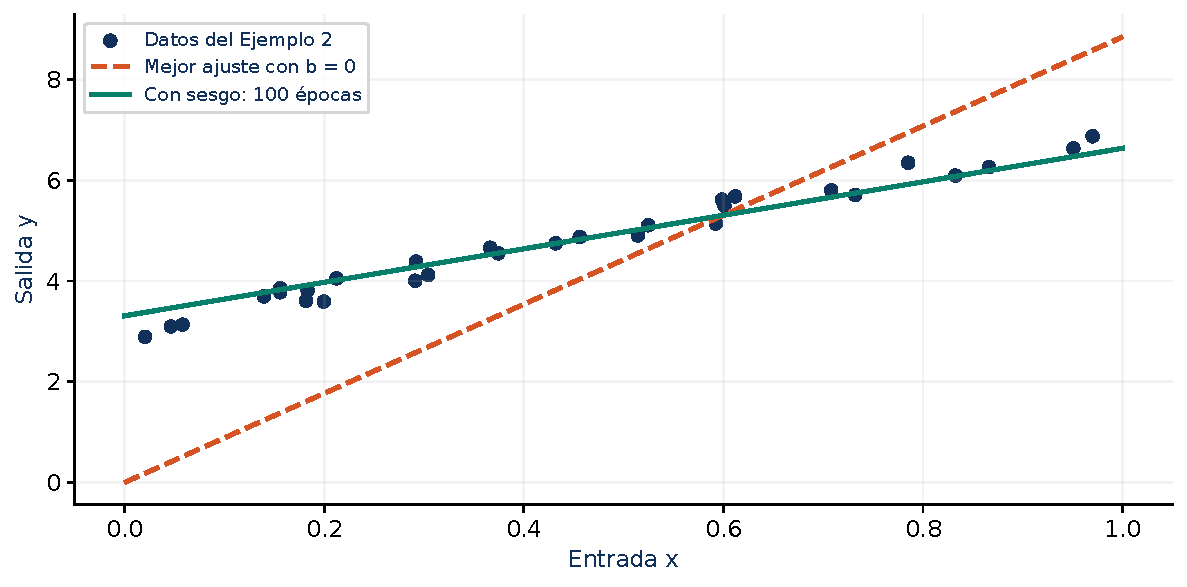
\includegraphics[width=0.72\textwidth,height=3.9cm,keepaspectratio]{efecto_sesgo.pdf}
    \actividad{Compara antes de entrenar}{¿Podemos ajustar bien estos datos si obligamos a la recta a pasar por el origen?}
    \note{Notebook: Ejemplo 2, celdas 22 a 33. La recta naranja es el óptimo de mínimos cuadrados con b=0; no es una mala inicialización. La verde corresponde a 100 épocas del notebook con sesgo entrenable. Esperar valores cercanos a w=4,b=3, sin exigir coincidencia exacta.}
\end{frame}

\begin{frame}[fragile]{Experimento 2: pesos iniciales distintos}
    \begin{caja}[greenbox]
        En el \textbf{Ejemplo 2}, conserva $X,y$ y usa la misma tasa y el mismo número de épocas.
    \end{caja}
\begin{lstlisting}
for semilla in [0, 42, 123]:
    w, b = fit(X, y, lr=0.1, epochs=100,
               random_state=semilla, verbose=False)
    print(semilla, w, b, L(s(a(X, w, b)), y))
\end{lstlisting}
    \actividad{Registra y explica}{¿Los resultados coinciden tras 100 épocas? Repite con 1000. ¿Qué cambió?}
    \note{Cambiar solo la semilla de fit, no volver a generar los datos con otra semilla. El problema cuadrático de estos datos tiene un único mínimo y una tasa estable permite converger hacia él; a un número finito de épocas puede haber diferencias. No extender esta conclusión a todas las redes neuronales.}
\end{frame}

\begin{frame}[fragile]{Extensión práctica: entrenamiento por bloques}
    \textbf{Regresamos al Ejemplo 1:} el bloque final usa $\hat y=wx$ y $b=0$.
\begin{lstlisting}
for lote in [30, 10, 1]:
    w, b = fit(X, y, lr=0.1, epochs=50,
               batch_size=lote, verbose=False)
    print(lote, w, L(s(a(X, w, b)), y))
\end{lstlisting}
    \begin{caja}[orangebox]
        \textbf{Antes de comparar: cuenta las actualizaciones.}\par\smallskip
        Con 50 épocas: lote 30 $\to$ 50 pasos; lote 10 $\to$ 150 pasos;
        lote 1 $\to$ 1500 pasos.
    \end{caja}
    \medskip
    \small Misma cantidad de épocas no implica el mismo número de actualizaciones.
    \note{Extensión opcional si falta tiempo. Ejecutar primero la celda completa que redefine datos y funciones en Entrenamiento por bloques (celda 36). El orden de las muestras es fijo. No afirmar que lote 1 siempre es mejor basándose en esta comparación.}
\end{frame}



\begin{frame}{Resumen: de una neurona a las próximas clases}
    \begin{columns}[T]
        \begin{column}{0.48\textwidth}
            \begin{caja}[greenbox]
                \textbf{Lo aprendido hoy}\par\medskip
                \small
                \begin{itemize}
                    \item Una neurona combina entradas mediante pesos y sesgo, y aplica una activación.
                    \item Con identidad, $\hat y=\bm w^\top\bm x+b$: un modelo para regresión lineal.
                    \item La pérdida mide el error; el gradiente indica cómo cambia con los parámetros.
                    \item Aprender es actualizar pesos y sesgo en dirección $-\nabla\mathcal L$, con una tasa adecuada.
                \end{itemize}
            \end{caja}
        \end{column}
        \begin{column}{0.49\textwidth}
            \begin{caja}
                \textbf{Lo que construiremos sobre esta base}\par\medskip
                \small
                \textbf{Lunes 30: clasificación.} Sigmoide y softmax; elegir la activación de salida y la pérdida según las clases.\par\medskip
                \textbf{Martes 1: perceptrón multicapa.} Componer capas con activaciones no lineales para aprender relaciones más complejas.\par\medskip
                \textbf{Miércoles 2: entrenamiento.} Retropropagación para calcular gradientes; optimizadores y regularización para mejorar el aprendizaje y la generalización.
            \end{caja}
        \end{column}
    \end{columns}
    \medskip
    \note{Antes de cerrar, pedir que expliquen con sus palabras qué cambia al entrenar y qué papel tienen la activación, la pérdida y la tasa de aprendizaje. Las próximas clases mantienen este ciclo: cambian las salidas y pérdidas para clasificación, se componen más capas y se calculan sus gradientes con la regla de la cadena. Recordar que reducir el error de entrenamiento no garantiza acertar en datos nuevos; esa distinción motivará la validación y la regularización. Contenidos futuros tomados de las guías Clase13.pdf, Clase14.pdf y Clase15.pdf.}
\end{frame}

\end{document}
